\documentclass[11pt]{article}
\usepackage[margin=0.82in]{geometry}
\usepackage[T1]{fontenc}
\usepackage{lmodern}
\usepackage{microtype}
\usepackage{graphicx}
\usepackage{booktabs}
\usepackage{tabularx}
\usepackage{array}
\usepackage{amsmath,amssymb}
\usepackage{xcolor}
\usepackage{listings}
\usepackage{hyperref}
\usepackage{float}
\usepackage{enumitem}
\usepackage{fancyhdr}
\usepackage{pgfplots}
\pgfplotsset{compat=1.18}
\usepgfplotslibrary{groupplots}
\usetikzlibrary{positioning}
\hypersetup{colorlinks=true,linkcolor=blue!45!black,urlcolor=blue!45!black}
\pagestyle{fancy}
\fancyhf{}
\lhead{Pure EDSL asset market}
\rhead{30-period pilot}
\cfoot{\thepage}
\setlength{\headheight}{14pt}
\definecolor{codebg}{HTML}{F6F8FA}
\definecolor{codekw}{HTML}{2457A6}
\definecolor{codestr}{HTML}{A31515}
\definecolor{codecom}{HTML}{547547}
\lstset{language=Python,basicstyle=\ttfamily\scriptsize,backgroundcolor=\color{codebg},
  keywordstyle=\color{codekw}\bfseries,stringstyle=\color{codestr},
  commentstyle=\color{codecom}\itshape,showstringspaces=false,breaklines=true,
  frame=single,rulecolor=\color{black!18},columns=fullflexible,
  numbers=left,numberstyle=\tiny\color{black!45},numbersep=7pt,
  xleftmargin=1.7em,framexleftmargin=1.3em,aboveskip=5pt,belowskip=8pt}
\newcommand{\code}[1]{\texttt{\small #1}}
\title{\vspace{-1.1em}A 30-Round Asset Call Market as a Pure EDSL State Machine}
\author{Replication note}
\date{October 2026}

\begin{document}
\maketitle
\begin{abstract}
This note documents a 30-period, 12-trader asset market implemented as an EDSL
\code{Machine}. The market mechanics---order admission, price-time priority,
uniform-price clearing, account transfers, interest, dividends, and terminal
redemption---are expressed in the Machine's serializable expression language.
The machine declares \code{algorithms=()}, so the market does not delegate
these operations to a custom Python algorithm or to EDSL's native call-market
factory. One completed \code{gpt-4o} pilot produced 360 trader decisions and
settled all 30 periods. Eight units traded in five periods, at prices from
\$15.00 to \$15.14. This is a documented pilot, not a statistical replication:
one market is insufficient to estimate the paper's market-level outcomes.
\end{abstract}

\tableofcontents
\newpage

\section{The experiment}
The experiment ports a baseline multi-period asset market into a dedicated
study directory. It contains
the Python authoring code, prepared workflow, completed run database, flat
analysis outputs, and this report. The run analyzed here is \code{pilot\_02},
seed 153101, using \code{gpt-4o} through EDSL's OpenAI service. The run completed
360 of 360 trader interviews, 30 of 30 clearings, and 30 of 30 settlements.

There are 12 traders, each starting with \$100 and four shares, for 48 shares
in total. In each of 30 periods, every trader submits one sealed buy, sell, or
hold decision. A buy order's requested units are limited by available cash at
the submitted limit price; a sell order is limited by current inventory. There
is no borrowing or short selling. Each period, every share pays a common
dividend, either \$0.40 or \$1.00 with equal probability. Cash earns 5 percent
interest per period. After period 30's interest and dividend, each remaining
share is redeemed for \$14.

Four traders receive a value-buyer instruction, four a value-seller
instruction, and four a flexible-value instruction. The instructions describe
trading tendencies, not hard-coded trading policies. Each model interview sees
the trader's current account and history plus the public market tape, and
returns four price forecasts and one order decision. Price limits are requested
in integer cents to avoid floating point conversion inside the market logic.

\section{Machine definition}
\subsection{State and transitions}
We can describe the machine as
\[
  M=(X, C, A, V, \delta, \mathcal{K}),
\]
where \(X\) is the typed mutable state, \(C\) is the constant data embedded
when the Machine is authored, \(A\) is the set of named commands, \(V\) is the
agent-facing view, \(\delta\) is the command transition semantics, and
\(\mathcal{K}\) is the set of registered runtime algorithms. Here
\(\mathcal{K}=\varnothing\). EDSL's standard interpreter evaluates the
serializable expressions in \(\delta\); the absence of callbacks does not mean
the Machine runs without an interpreter.

The mutable state is
\[
X_t=(\text{accounts}_t,\text{orders}_t,\text{clearing}_t,
\text{orderLog}_t,\text{tape}_t, p_t, \ell_t, f_t),
\]
with per-trader cash in cents, share inventory, and private history inside
\code{accounts}; current-period submitted orders in \code{orders}; the pending
allocation in \code{clearing}; public history in \code{order\_log} and
\code{tape}; current period \(p_t\); last transaction price \(\ell_t\); and
terminal flag \(f_t\). The view exposes the public tape and the current trader's
own account, but does not expose other traders' private account histories.
The initial state has 12 identical accounts, 10,000 cents and four shares per
account, period 1, reference price 1,400 cents, empty orders and histories, and
\(f_1=\text{false}\).

There are three transitions, all represented as \code{Command} expressions:
\begin{enumerate}[leftmargin=2em,itemsep=2pt]
  \item \textbf{\code{submit\_order}(i,t,d)} requires an unfinished market, the
  current period, a known trader, and no order already submitted by that trader
  in this period. It validates hold versus buy/sell fields, caps buy quantity at
  \(\min(q_{requested},\lfloor C_i/L_i\rfloor,48)\), and caps sell quantity at
  \(\min(q_{requested},S_i)\). It stores the accepted decision. The submission
  does not directly mutate cash or shares.
  \item \textbf{\code{clear\_orders}(t)} requires exactly 12 submitted orders
  and no existing pending clearing. It expands each accepted order into unit
  bids or asks, sorts them by price and seeded priority, and computes the
  maximum crossing volume. It stores the resulting matched units, fills, and
  a single uniform transaction price in \code{clearing}.
  \item \textbf{\code{settle}(t)} requires a pending clearing. It applies cash
  and share transfers, interest, dividends, histories, the public tape, and
  (in period 30) redemption. It clears the order book and pending allocation,
  advances the period, and sets \code{finished} after the final period.
\end{enumerate}

\subsection{Allocation and uniform price}
Expand each admitted order of size \(q\) into \(q\) unit orders. Let the ranked
bid limits be \(b_1\ge b_2\ge\dots\), and ask limits \(a_1\le a_2\le\dots\).
Ties use a seeded period-specific trader priority; unit index makes multiple
units from one trader deterministic. The matched quantity is
\[
  Q_t=\max\bigl(\{0\}\cup\{q\in\{1,\ldots,\min(n_b,n_a)\}:b_q\ge a_q\}\bigr),
\]
with the empty match represented by \(Q_t=0\). If \(Q_t>0\), all matched
units trade at
\[
  P_t=\operatorname{round}_{\text{half-up},\,\text{cent}}\!\left(
       \frac{b_{Q_t}+a_{Q_t}}{2}\right).
\]
Thus the price is the rounded midpoint of the marginal matched bid and ask.
The highest bids and lowest asks receive the fills. Unfilled orders expire at
settlement. If no units cross, no transaction price is recorded and the last
transaction price remains the public reference price.

For trader \(i\), define \(x_{it}\) as filled purchases minus filled sales,
and \(C^-_{it},S^-_{it}\) as cash and inventory before the trade. At a trade
price \(P_t\) measured in cents, the post-trade balances are
\[
  \widetilde C_{it}=C^-_{it}-x_{it}P_t,\qquad
  \widetilde S_{it}=S^-_{it}+x_{it}.
\]
The period income and end balances are
\[
  I_{it}=\operatorname{round}_{\text{half-up}}(0.05\widetilde C_{it}),\quad
  D_t\in\{40,100\}\text{ cents},\quad
  C^+_{it}=\widetilde C_{it}+I_{it}+D_t\widetilde S_{it}+R_{it},
\]
where \(R_{it}=1400\widetilde S_{it}\) in period 30 and zero otherwise.
After redemption, the period-30 inventory is set to zero. All arithmetic for
prices, cash, interest, dividends, and redemption is performed in integer
cents; ratios explicitly specify floor or half-up rounding.

\subsection{Fair-value benchmark}
The expected dividend is \$0.70 per share per period, exactly five percent of
the \$14 redemption value. Under risk-neutral discounting at the cash interest
rate, the value at the beginning of any period with \(n\) dividend payments
remaining is
\[
  V_n=\sum_{k=1}^{n}\frac{0.70}{(1.05)^k}
      +\frac{14}{(1.05)^n}=14.
\]
This \$14 benchmark is a useful reference for interpreting prices, conditional
on the stated common dividend process, risk-neutral valuation, and the 5 percent
cash rate. It is not a claim that all model traders share those assumptions.

\section{How one market run proceeds}
The workflow uses one session-scoped \code{SharedStateMap} and one instance of
the Machine for the full market. Each period has three ordered workflow steps:
\begin{enumerate}[leftmargin=2em,itemsep=2pt]
  \item \textbf{Orders:} the 12 trader role members each read the same current
  shared state, but receive an account view personalized to their identity.
  Their responses are written with \code{submit\_order}. Interviews can run
  concurrently, while each writes only its own map entry.
  \item \textbf{Clearing:} after all trader interviews finish, a scripted
  exchange participant invokes \code{clear\_orders}. The question text asks
  for no arithmetic; the actual allocation and price are evaluated by the
  Machine expression.
  \item \textbf{Settlement:} the exchange step invokes \code{settle}. It
  applies the allocation and income and closes the period's book.
\end{enumerate}
The next period depends on completion of settlement. This sequence repeats
30 times, giving 90 workflow steps, 360 trader interviews, 30 clearing
transitions, and 30 settlement transitions. The persisted state log contains
360 reads and 420 writes: one decision write for each trader interview, one
clearing write and one settlement write per period.

\begin{figure}[H]
\centering
\resizebox{\linewidth}{!}{%
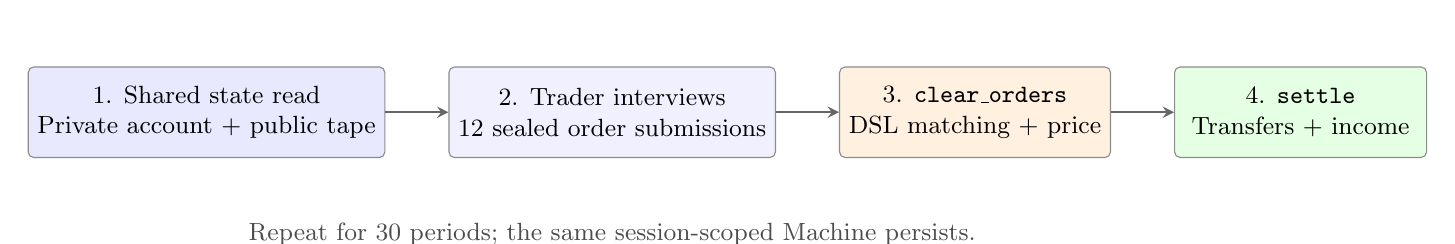
\begin{tikzpicture}[>=stealth, node distance=8mm,
  flowbox/.style={draw=black!45, rounded corners=2pt, minimum width=3.2cm,
    minimum height=1.15cm, align=center, font=\small}]
  \node[flowbox, fill=blue!9] (read) {1. Shared state read\\Private account + public tape};
  \node[flowbox, fill=blue!6, right=of read] (orders) {2. Trader interviews\\12 sealed order submissions};
  \node[flowbox, fill=orange!12, right=of orders] (clear) {3. \code{clear\_orders}\\DSL matching + price};
  \node[flowbox, fill=green!10, right=of clear] (settle) {4. \code{settle}\\Transfers + income};
  \draw[->, thick, black!60] (read) -- (orders);
  \draw[->, thick, black!60] (orders) -- (clear);
  \draw[->, thick, black!60] (clear) -- (settle);
  \node[below=7mm of orders, align=center, font=\small\color{black!70}]
    {Repeat for 30 periods; the same session-scoped Machine persists.};
\end{tikzpicture}
}%
\caption{One period of the workflow. The order interviews can run in parallel;
clearing and settlement wait on their respective predecessor steps.}
\end{figure}

\section{Implementation in EDSL}
The expression builders assemble serializable tree nodes. Python is used to
author the tree and to materialize the seeded exogenous schedules. The schedule
is part of the Machine constants, so no Python random draw or market callback
is needed while executing a transition. The builder calls \code{validate()}
before returning the Machine.

The source's unit expansion and crossing scan make the matching rule explicit:

\lstinputlisting[firstline=112,lastline=184,caption={Source excerpt: expanding and ranking unit orders, then scanning crossing bids and asks.}]{machine_definition.py}

The actual Machine declaration below defines typed state fields, command
preconditions, and state effects. These are Python builder calls; the market
logic within command effects is still encoded as EDSL expressions, not an
imperative callback body.

\lstinputlisting[firstline=450,lastline=493,caption={Source excerpt: seeded constants, initial accounts, and typed state.}]{machine_definition.py}

\lstinputlisting[firstline=493,lastline=562,caption={Source excerpt: the three Machine commands, agent view, empty algorithm registry, and validation.}]{machine_definition.py}

\section{Pilot results}
\subsection{Completion and activity}
All 360 interviews were completed and all 30 periods settled. The Machine
finished in period 31 with no pending orders, zero remaining shares, and 48
redeemed shares. The run logged 360 shared-state reads and 420 writes, exactly
matching the workflow's planned decision and market transition counts.

There were 213 buy decisions, 89 sell decisions, and 58 holds. Those counts
are choices, not executions. Only eight units traded, across five periods;
25 periods had no transaction. The market's active trading interval was
periods 10 through 14. The price rose in each of these five periods, from
\$15.00 to \$15.14; afterward the last transaction price was carried forward
as the tape reference, but it was not a new market quote.

\begin{figure}[H]
\centering
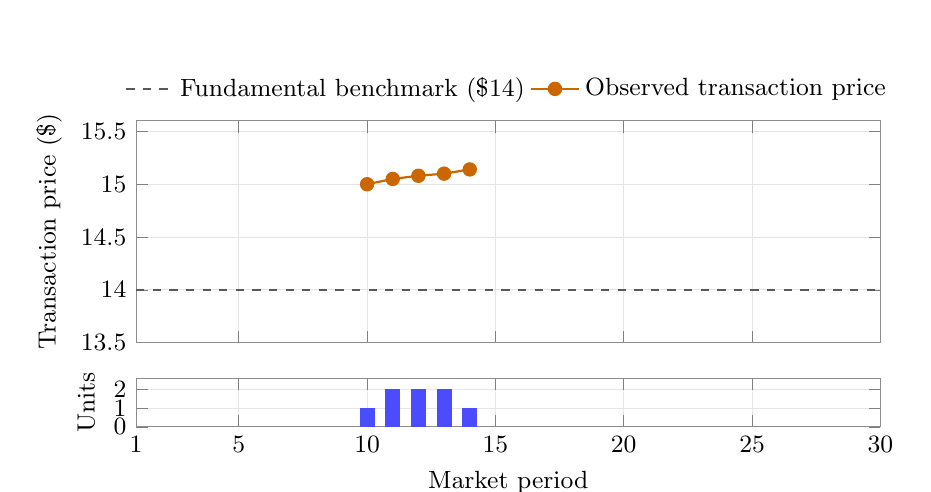
\begin{tikzpicture}
\begin{groupplot}[group style={group size=1 by 2,vertical sep=0.45cm},
  width=0.91\linewidth]
\nextgroupplot[height=4.4cm,
  xmin=1,xmax=30,ymin=13.5,ymax=15.6,
  ylabel={Transaction price (\$)},
  xtick={1,5,10,15,20,25,30},xticklabels=\empty,
  grid=major,grid style={black!10},
  axis line style={black!45},tick label style={font=\small},
  label style={font=\small},legend style={draw=none,fill=none,font=\small,
    at={(0.5,1.04)},anchor=south,legend columns=2}]
  \addplot[black!65,dashed,thick,domain=1:30] {14};
  \addlegendentry{Fundamental benchmark (\$14)}
  \addplot[orange!80!black,thick,mark=*,mark size=2.2pt]
    coordinates {(10,15.00) (11,15.05) (12,15.08) (13,15.10) (14,15.14)};
  \addlegendentry{Observed transaction price}
\nextgroupplot[height=2.2cm,
  xmin=1,xmax=30,ymin=0,ymax=2.6,
  xlabel={Market period},ylabel={Units},
  xtick={1,5,10,15,20,25,30},ytick={0,1,2},
  grid=major,grid style={black!10},
  axis line style={black!45},tick label style={font=\small},
  label style={font=\small}]
  \addplot[ybar,bar width=5pt,fill=blue!70,draw=blue!70]
    coordinates {(10,1) (11,2) (12,2) (13,2) (14,1)};
\end{groupplot}
\end{tikzpicture}
\caption{The five transaction observations and traded quantity. Periods
without a marker had no transaction; the tape carries the last transaction
price as a reference, not as a new clearing price.}
\end{figure}

\begin{table}[H]
\centering
\begin{tabular}{rrrr}
\toprule
Period & Transaction price & Units & Difference from \$14 \\
\midrule
10 & \$15.00 & 1 & 7.1\% \\
11 & \$15.05 & 2 & 7.5\% \\
12 & \$15.08 & 2 & 7.7\% \\
13 & \$15.10 & 2 & 7.9\% \\
14 & \$15.14 & 1 & 8.1\% \\
\midrule
All trades & Mean \$15.074 & 8 & 7.7\% above benchmark \\
\bottomrule
\end{tabular}
\caption{Observed transaction prices. Each row is one period's uniform price;
the total quantity matched was eight units.}
\end{table}

\subsection{Trading styles and allocation}
The model followed the broad direction of its assigned styles, although these
were instructions rather than binding algorithms. The four value buyers made
117 buys and three holds. Value sellers made 87 sells and 33 holds. Flexible
value traders made 96 buys, 22 holds, and two sells. In this run, the flexible
role leaned strongly toward buying. The 8 purchased units went to flexible
traders; 8 units were sold by two value sellers. Every other share remained
with its initial holder and was redeemed at the end.

\begin{figure}[H]
\centering
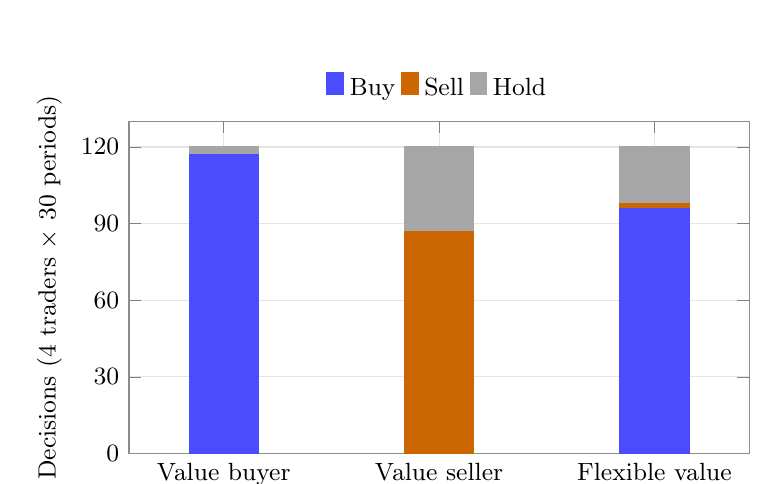
\begin{tikzpicture}
\begin{axis}[ybar stacked,bar width=25pt,width=0.78\linewidth,height=5.8cm,
  ylabel={Decisions (4 traders $\times$ 30 periods)},
  symbolic x coords={buyer,seller,flexible},
  xtick=data,xticklabels={Value buyer,Value seller,Flexible value},
  ymin=0,ymax=130,ytick={0,30,60,90,120},
  enlarge x limits=0.22,grid=major,grid style={black!10},
  axis line style={black!45},tick label style={font=\small},
  label style={font=\small},legend style={draw=none,fill=none,
    at={(0.5,1.03)},anchor=south,legend columns=3,font=\small}]
  \addplot[fill=blue!70,draw=blue!70] coordinates {(buyer,117) (seller,0) (flexible,96)};
  \addlegendentry{Buy}
  \addplot[fill=orange!80!black,draw=orange!80!black] coordinates {(buyer,0) (seller,87) (flexible,2)};
  \addlegendentry{Sell}
  \addplot[fill=black!35,draw=black!35] coordinates {(buyer,3) (seller,33) (flexible,22)};
  \addlegendentry{Hold}
\end{axis}
\end{tikzpicture}
\caption{Actions by assigned style, aggregated across each role's four traders
and all 30 periods.}
\end{figure}

Total trader cash after redemption was \$8,150.35. Final balances ranged from
\$661.18 to \$690.67. All traders started with \$100 and four shares, whose
combined terminal redemption value was \$672 per trader before interest,
dividends, and trading. Two value sellers sold all four of their shares before
redemption; flexible traders bought those eight shares. The spread of final
cash thus reflects dividend and interest receipts, plus the timing and price
of those transfers.

\subsection{Forecasts}
Mean reported forecasts were \$14.903 for the current-period price, \$15.005
two periods ahead, \$15.135 five periods ahead, and \$15.311 ten periods ahead.
Mean absolute errors against realized transaction prices were \$0.184,
\$0.566, \$0.710, and \$0.503, respectively. These errors are computed only
when a transaction exists at the forecast target: the sample sizes are 60 for
horizons 0, 2, and 5, and 48 for horizon 10. They are not errors over all
forecasts or over unobserved no-trade periods. Because prices were observed in
only five periods, these diagnostics should be read as sparse pilot summaries.

\section{What the pilot says about the implementation}
\paragraph{The DSL carried the market mechanics.} The Machine declares three
commands, typed state and inputs, preconditions, and effects. The market's
allocation, price, settlement, interest, dividend, and redemption are all
composed from built-in expressions. In the experiment's metadata and serialized
definition, the algorithm list is empty. This is direct evidence that this
version is not a wrapper around the native \code{call\_market} factory and does
not subclass that market's transition implementation.

\paragraph{Machine serialization is useful, with a boundary.} The definition
serializes to JSON and contains its seeded schedules and expression trees. It
can therefore be inspected, stored, validated, and replayed by an EDSL runtime.
The runtime remains necessary to interpret the expression language and enforce
command preconditions; JSON alone is a data representation, not an executable
interpreter.

\paragraph{The larger per-operation budget is necessary for full-history state.}
The default one-million-step interpreter ceiling was exhausted by a late-round
transition in an earlier full-horizon attempt. The experiment sets the ceiling
to ten million steps. The Machine deliberately retains every order and each
trader's period history for inspection, so transition work grows over time.
The deterministic 30-period mechanics smoke and this live run both reached
terminal completion with the larger limit.

\paragraph{Model inference dominates observed runtime.} Log timing for this
pilot showed roughly 38--40 seconds for a batch of 12 trader interviews, while
the clearing transition averaged about 1.47 seconds and settlement about 1.85
seconds. The two DSL transitions therefore took about 3.3 seconds per round,
small beside the model calls. The shared-state version adds measurable
expression evaluation and state-log work, but the observed end-to-end delay is
primarily the language-model inference.

\section{Interpretation and next replication steps}
This run establishes that the full-period mechanics can be encoded in the
Machine expression language and executed through the shared-state workflow,
including account constraints and terminal cash-out. It does not establish
that the market reproduces the paper's behavioral or price outcomes. The market
traded only eight units, and prices were observed only in five periods. The
15-cent range in those five prints is descriptive; with one seeded market it
cannot be treated as an estimate of typical price convergence, mispricing, or
volume.

A paper-level comparison should run multiple independent markets and compare
the same market-level statistics reported in the source paper, with uncertainty
at the market level. It should also inspect order submission, fill rates,
trading volume, price paths, and trader earnings by strategy. Forecast metrics
should continue to distinguish transaction-observed targets from periods with
no transaction. The saved run is suitable as a mechanics and workflow pilot;
its eight-unit tape is too sparse to support stronger economic conclusions.

\appendix
\section{Workflow source: launching and running the experiment}
The experiment creates a single Machine-backed shared state, binds the trader
role to a language model and the exchange role to scripted answers, then chains
orders, clearing, and settlement for each period. The clearing and settlement
answers are merely workflow responses; all effects come from the attached
Machine commands.

\lstinputlisting[firstline=99,lastline=135,caption={Source excerpt: agents, session-scoped Machine state, and execution-plan bindings.}]{experiment.py}

\lstinputlisting[firstline=137,lastline=205,caption={Source excerpt: chained order, clearing, and settlement steps, and WorkflowExperiment construction.}]{experiment.py}

The command used to launch the completed pilot was:
\begin{lstlisting}[language=bash,basicstyle=\ttfamily\scriptsize,backgroundcolor=\color{codebg},frame=single,breaklines=true]
python3 edsl_replication/studies/asset_market_pure_edsl_30r/experiment.py \\
  --output edsl_replication/studies/asset_market_pure_edsl_30r/pilot_02
\end{lstlisting}
The run artifacts include the serialized specification and experiment,
workflow and state databases, completion record, model-call log, and the
derived CSV and JSON summaries.

\section{Run environment and operational notes}
The only run analyzed here is the successful \code{pilot\_02} market. The
prepared workflow and persisted database confirm 360 decisions and 30 complete
periods. An earlier full-horizon mechanics attempt reached the default
one-million-step expression ceiling late in the run; the 10-million-step
configuration allowed the deterministic smoke and the model-backed market to
complete. Initial local object-cache permission errors were retried and are not
part of the economic results. They did not reduce the completed sample.

\section{Reproducibility files}
The implementation and outputs are stored alongside this PDF:
\begin{itemize}[leftmargin=2em,itemsep=2pt]
  \item \code{machine\_definition.py}: the Machine and serializable expression trees.
  \item \code{experiment.py}: agents, questions, shared state, workflow, and run entry point.
  \item \code{pilot\_02/specification.json}: prepared serializable workflow and machine.
  \item \code{pilot\_02/results\_summary.json}: aggregate counts and descriptive statistics.
  \item \code{pilot\_02/round\_summary.csv}: period-level tape and income fields.
  \item \code{pilot\_02/trader\_summary.csv}: strategy, final balances, orders, and fills by trader.
\end{itemize}
The analysis script \code{analyze\_run.py} regenerates the two CSV files and
summary JSON from the saved state and workflow databases. For a new independent
market, use a fresh output directory and a different seed. The deterministic
mechanics-only smoke is available as \code{smoke\_run.py}.

\end{document}
